\documentclass[a4paper, 11pt]{article}

%Handige usepackages voor essays
\usepackage{graphicx} % Required for including pictures
\usepackage{wrapfig} % Allows in-line images

%Standaard usepackages
\usepackage{pdfsync}
\usepackage[english]{babel}
\usepackage{fullpage}
\usepackage{amsmath}
\usepackage[table]{xcolor}
\usepackage{caption}
\usepackage{subcaption}
\usepackage{float}
\usepackage{verbatim}
\usepackage{eso-pic}
\usepackage[toc,page]{appendix}
\usepackage[linkbordercolor={white}]{hyperref}
\usepackage{nameref}
\usepackage{listings}

\makeatletter
\renewcommand{\@listI}{\itemsep=0pt} % Reduce the space between items in the itemize and enumerate environments and the bibliography

\renewcommand{\maketitle}{ % Customize the title - do not edit title and author name here, see the TITLE block below
\begin{flushright} % Right align
{\LARGE\@title} % Increase the font size of the title

\vspace{50pt} % Some vertical space between the title and author name

{\large\@author} % Author name 1
\\\@date % Date

\vspace{40pt} % Some vertical space between the author block and abstract
\end{flushright}
}

%----------------------------------------------------------------------------------------
%	TITLE
%----------------------------------------------------------------------------------------

\title{\textbf{Internet of Things }\\ % Title
Developing an optimal wireless power transfer system for a real-world low power LED wristband application} % Subtitle

\author{\textsc{Muhammad Wasif \\ 
Imara Speek} % Author
\\{\textit{Delft University of Technology}}} % Institution

\date{\today} % Date

%----------------------------------------------------------------------------------------

\begin{document}

\maketitle % Print the title section

%----------------------------------------------------------------------------------------
%	ABSTRACT AND KEYWORDS
%----------------------------------------------------------------------------------------

%\renewcommand{\abstractname}{Summary} % Uncomment to change the name of the abstract to something else

\begin{abstract}
Morbi tempor congue porta. Proin semper, leo vitae faucibus dictum, metus mauris lacinia lorem, ac congue leo felis eu turpis. Sed nec nunc pellentesque, gravida eros at, porttitor ipsum. Praesent consequat urna a lacus lobortis ultrices eget ac metus. In tempus hendrerit rhoncus. Mauris dignissim turpis id sollicitudin lacinia. Praesent libero tellus, fringilla nec ullamcorper at, ultrices id nulla. Phasellus placerat a tellus a malesuada.
\end{abstract}

\hspace*{3,6mm}\textit{Keywords:} Wireless power transfer, low power, real-world application % Keywords

\vspace{30pt} % Some vertical space between the abstract and first section

%----------------------------------------------------------------------------------------
%	ESSAY BODY
%----------------------------------------------------------------------------------------

\section{Introduction}
\label{sec:intro}
% Something about the assignment
% our interpretation
% how can this be achieved
% how can it be used right now, in a real world example
% how are we contributing to this example
%
Although wireless power transfer systems are already widely applied in stationary household equipment, current research offers a tremendous amount of possibilities that can change our perception of energy usage. In an ideal world we would no longer have to concern about wires and depleting batteries. A collection of wireless power transmitters would be able to charge all our products wirelessly, enabling a completely mobile and energy independent workspace or living environment. This report will introduce a reusable mobile real-world low power application that utilizes a wireless power transfer system to eliminate the need for changing batteries. Introducing wireless power transfer techniques into the world of reusable high quality products will greatly reduce the environmental risks of the product and thus increase product value.

In this report we will briefly discuss our choosen paper \cite{paper} and present a working product that extends the basic ideas discussed in the paper. As the paper itself did not discuss any \emph{Internet of Things} aspects to their idea, we present a scenario where both techniques could be fully utilized. The concurring product to match this scenario is based on the \emph{Drome Surround light} \cite{drome}. The drome is a LED wristband powered by a battery to be worn at concerts that enriches the involvement of the audience by including them into a lightshow and can run for 5 hours after it is switched on. The dromes can be reused after each show by replacing the batteries and this report will focus on eliminating this need. First we will focus on the choosen paper in Section \ref{sec:related} and some prior knowledge in Section \ref{sec:prior}. Section \ref{sec:idea} will discussed our start-up based idea in a scenario, initial wireless transfer system, a state analysis and the concurring protocols. Section \ref{sec:analysis} will go deeper into the system design by analyzing our electonic model, model the battery life, charging profile and the charge to discharge ratio. In Section \ref{sec:proposed} the proposed final system design and the internet of things will be discussed. We will conclude our results in Section \ref{sec:results} and present the conclusion and future works in Section \ref{sec:conclusion} and \ref{sec:future}.

% introduction to what wireless power transfer solves --> an ideal world 
% how can this be achieved 
% how can it be used right now, in a real world example
% how are we contributing to this example

%------------------------------------------------

\section{Related work}
\label{sec:related}
% related work 
The assigned paper \cite{paper} presents an \emph{"Architectural analysis for wirelessly powered computing platforms"}. As we already discussed the downfalls of the paper thoroughly in class we will need go into too much details, but we will just present in what ways we extended the proposed idea in the paper. The authors of the paper provide a model for a single kind of wireless powered system. However, the system only assumes power requirements that includes constant voltage levels and do not include anything about constant current or power. Furthermore each wireless power packet is assumed to carry constant power and is recieved periodically while the period is known in advance. 

In our wireless powered system, the system components immensly differ from the system proposed in the related work. The system in the related work does not include any storage device apart from the small rectifying capacitor, which makes the system useless in the absence of wireless power. For this reason we included a supercapacitor and a battery and two main big storage components which can keep the system operational even in the absence of wireless power. Also, the related work made some unrealistic assumptions of the periodic reception of constant powered wireless energy packets which led us to make a completely different analytical model as disccused in Section 5. Consequently the related work only provides an intial guideline for wireless powered system, for more practical systems a completely new analytical model is required.      
 

% Firstly present the assigned project paper
% introduction to our idea evaluation
% why this idea and why not something else (how is it different)

%------------------------------------------------

\section{Prior knowledge}
\label{sec:prior}
Since the technolological advancements in materials. The gap between supercapacitor and the conventional batterys for large charge storage is reducing. Supercapacitor can charge really fast and have much longer life as compared to battery. Hence it is much usefull to use a supercapacitor then a battery. However, supercapacitors with the same size as of battery can hold about 10 times less energy than a Li-ion battery. The table below givee some comparsion between suppercapacitor and a Li-ion battery. In order to get the best out of both, one can combine both in parallel. 

%%%%%%%%%%%%%%%Table %%%%%%%%%%%%%%%%%



\begin{tabular*}{\textwidth}{@{\extracolsep{\fill}} |l|l|l|}
\hline
Characteristic & Supercapacitor & Li-ion Battery \\
\hline
Charge time & 1–10 seconds & 10–60 minutes \\
Cycle life & 1 million or 30,000h & 500 and higher \\
Cell voltage & 2.3 to 2.75 Volts & 3.6 to 3.7 Volts \\
Cost per Wh & Cost per Wh & $0.50-$1.00 (large system) \\
\hline
\end{tabular*}
\begin{center}
\textbf{ Table 1.} Comparison between Supercapacitor and a Battery \cite{superbattery}
\end{center}


% an introduction to wireless energy transfer, show some images
% something about quick charging and long battery life is often done
% How longer distances can be achieved in charging (hint that this is not possible with our project)

%-----------------------------------------------

\section{Description of the proposed idea} 
\label{sec:idea}
decription idea
start up based product
add some internet of things
% graded on very innovative idea,
% clear application 
% startup-based idea

% short introduction to the scenario
% how does this include the priorly introduced paper

\subsection{Working towards a realization}
\label{sec:realize}
Our major goal is to provide with an efficient solution that best meet the challenges in battery charging systems using wireless power transfer.
Those challenges include:
\begin{enumerate}
\item Charging the battery as quickly as possible. 
Though batteries can store large amount of charge but unfortunately there is a limit to how fast a battery can be charged and this limit gets smaller with the size (capacity) of a battery. Smaller the battery, smaller the charging current limit will be and exceeding this limit will deteriorate battery's life. To overcome this difficulty we proposed adding a super capacitor in parallel with a battery. Even though super capacitors can hold less amount of charge compared to the same size battery but they can be charged much faster \cite{IAmp}.
\item Providing long battery life with large charge to discharge ratio.
In our scenario we want to make the charging interval as small as possible which requires a need to store as much charging current as possible in this short interval and that makes the addition of super capacitor an ideal solution to overcome the battery charging limitation. During the charging interval, super capacitor can store large amount of charging current and then later use this current to charge the battery with slow pace. Which provides long battery life in terms of large charge to discharge ratio.
 
\item Working out efficient protocol for sharing the available charge.
%%%%%%%%%%%%%%%%%%%%%%%%%%%%%%%%%%%%%%%%%%%%%%%%%%%%%%%%%%%%%%%%%%%%%%

\end{enumerate}

% what are our goals --> quick charging and long battery life,a final product, IoT element and some protocols and computing policies 
% how will we achieve these goals --> decribe the set-up of the experiment
% tip of the iceberg, include some formulas

\subsection{Protocols concerning environmental impact features}
\label{sec:proto}
%
Charging protocols have to be designed to account for the state translations described in Section \ref{sec:states}. We considered three possible energy charging scenarios: an infinite network like design where all nodes should stay alive, a hop-to-hop spread of energy that uses inter-module detecting or charge requests or an interactive behavior to selectively share energy. To stimulate interaction through this application we choose to apply a scenario where a user can choose to act upon energy requests and share with friends, or strangers. This is the best suiting approach considering the environment of a festival where you can meet new people and can "share the love". 

Based on figure \ref{fig:states} we can determine all the possible state translation and the concurring protocols that are required. In this section we will generate pseudocode for the application that can be translated onto environment for an IC. For the IC we decided to choose the \emph{Arduino Pro Mini} \cite{promini}, a flexible small microcontroller for the arduino environment. For the real-world application we can fit the arduino in a relative small wristband.  As the recognitions of the RFID tag that is included in the internet of things part is a passive component of the wristband, it is not included into the code. 
\\
\lstinputlisting{ICiot/ICiot.ino}
%\lstinputlisting{pseudo.c}


%To handle these protocols, an IC has to be added. This way whenever the battery reached $V_{starve}$ it will send out a request for energy visually by litting a red LED embedded in the wristband. Neighbouring nodes can then choose to react on this or save their own energy. Whenever the battery dies, the user either has to verbally ask for energy or visit an energy bar.

% an introduction to what we need to take into account when designing for this real-world example
% include the state diagram 
% present Internet of Things ness

%-----------------------------------------------

\section{The proposed system design} 
\label{sec:proposed}
The Figure \ref{fig:design1} shows the proposed design of the system. The system includes a transmitter and a receiver with transmission and receiving coil respectively. The wireless power transmission works on the principle of magnetic induction \cite{IAmp}. The transmitter is powered up by a voltage source $V_i$ of 12 Volts capable of delivering 400 milli-Amps of $i_{in}$ current. $i_c$ is the constant current that is consumed by the transmitter circuitry and $i_s$ is the induction current which flows through the transmitter coil such that $i_{in} = i_c + i_s$ . $i_c$ is constant and depends on the transmitter inner circuitry power consumption, in our case $i_c = 100 milli-Amps $. $i_s$ depends on the distance between the two magnetically coupled coils, greater the distance smaller the $i_s$ will be. Another factor that $i_s$ could depend is on adding an iron core between the two coils, adding a core makes the magnetic coupling stronger and increases the $i_s$ which enhances an overall efficiency of the system.
The receiver circuit receives an induction voltage $V_r$, rectifies it through a rectifier containing a shotkey diode $D_r$ and a capacitor $C_r$. A shotkey diode is used in order to have a good frequency response at the range of $ 300-400 Khz$ the transmitter working frequency also shotkey has lower forward voltage drop. The rectified voltage is then fed to the voltage regulator that produces constant voltage $V_{reg} = 5 Volts$ .

\emph {determine $V_{starve}$, $V_{dead}$, $V_{full}$}
% graded for: complete code/schematics of the developed project
% code well documented and structures
% choices of used software, procedure and/or hardware well justified

% How we came to this design, including some references
% What we focussed on, which results do we want to achieve
% why we choose for these solutions, justify software, procedure and hardware
% Some schematics of the set up
% source code or pseudo code whether or not that is necessary

%----------------------------------------------

\section{Results}
\label{sec:result}
Figure \ref{fig:results} shows charge to discharge ratio from the practical system. Compared to the theoretical result shown in figure \ref{fig:crs} (a) a clear degradation can be noticed. The average value has been reduced from 6 to 4.75. This is due to two major reasons, the imperfection of practical components and the assumptions taken in theoretical model. In theoretical model we made the assumption that during the charge cycle there is no current flowing into the battery and $i_r \approx i_c $, where as in reality a small current is flowing into the battery hence producing the non ideality in the actual results.

%---------- Charge to Discharge ratio from the actual circuit
%
\begin{figure}[h!]
\centering
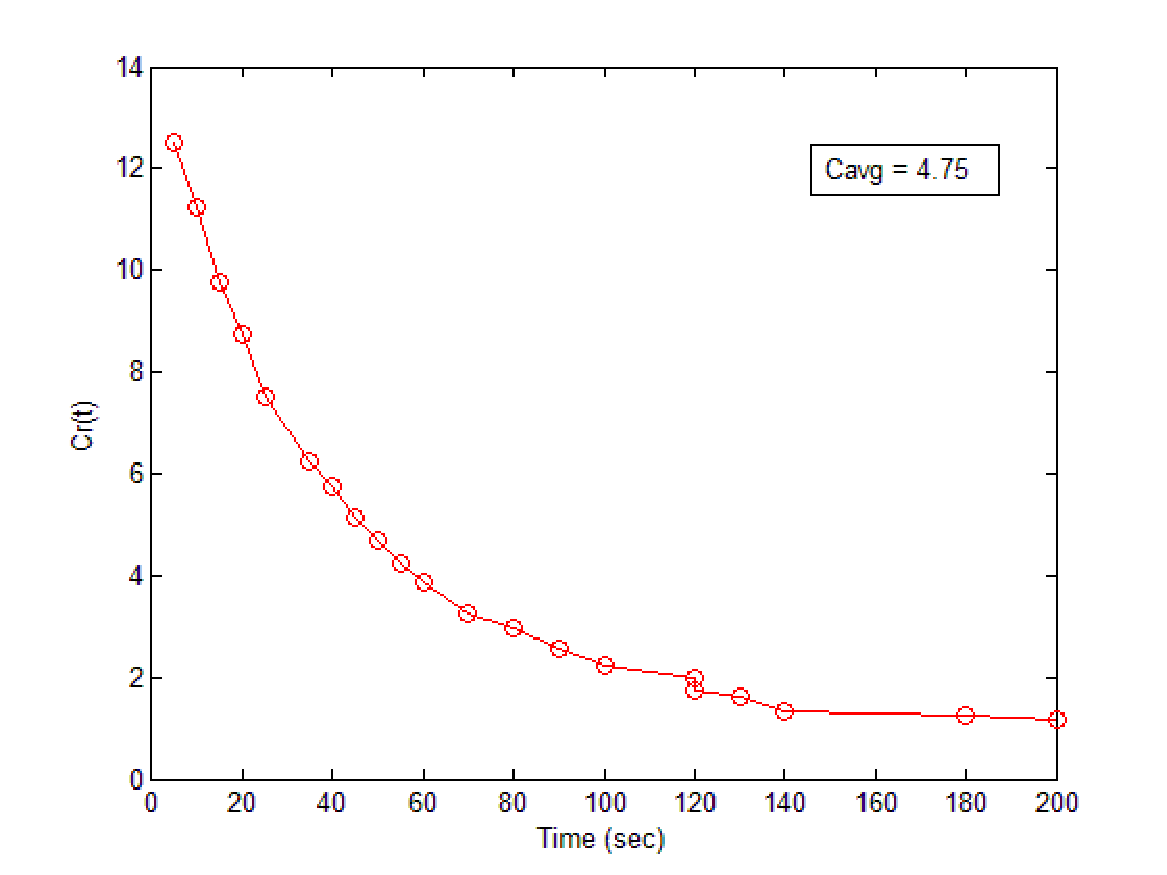
\includegraphics[width=0.8\textwidth]{results.pdf}
\caption{Charge to discharge Ratio}
\label{fig:results}
\end{figure}
%

%---------- The dimension figure goes here

\begin{figure}[h!]
\centering
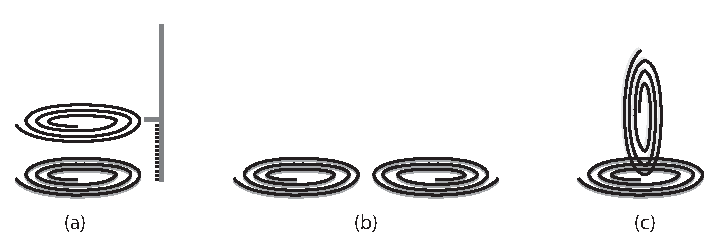
\includegraphics[width=0.9\textwidth]{dimension.pdf}
\caption{Orientations of the test set-up}
\label{fig:dimension}
\end{figure}

%-----------------------Table ----------------------------------------
\begin{tabular*}{\textwidth}{@{\extracolsep{\fill}} |l|l|}
\hline
Distance between two coils (cm) & Efficiency (\%) \\
\hline
0 & 70 \\
1 & 60 \\
2 & 50 \\
3 & 40 \\
4 & 30 \\
\hline
\end{tabular*}
\begin{center}
\textbf{ Table 2.} Distance vs Efficiency
\end{center}

% graded for a working demonstrator and fully operating system
% idea evaluated against state of the art solutions
% clear described methodology of experiment
% good handling of the results

% introduction to set up measurements 
% why this set up, why these measurements
% evaluation of model against state-of-the art
% nice graphical representations of results
% some details about charging time, performance, battery life
% critical analysis of experiments and how this impacts our project

%----------------------------------------------

\section{Conclusion}
\label{sec:conclusion}
A wireless power transmission system based on the principal of magnetic coupling was used and analyzed. A wristband system application was purposed and additional components were added to aid the feasibility of that application. The performance in terms of efficiency and charge to discharge ratio of the wristband system was analyzed. Additional components, super capacitor and high power constant current charger, were purposed to further enhance the performance. Based on different scenarios, protocols were introduced to efficiently define the complete working of the application and the Arduino platform was used for the realization of these protocols. Finally some comparisons were made between theoretical and practical results and the reasons for their differences were discussed.
% graded on: concise summary using measurable units
% gives prospects for further evaluation
% enlist surprising/non-trivial lessons learned

% a concluding paragraph about everything that we did
% A critical analysis of our project and its feasibility
% a critical analysis on our results
% surprising lessons learned
% some future guidelines

%----------------------------------------------------------------------------------------
%	BIBLIOGRAPHY
%----------------------------------------------------------------------------------------

\bibliographystyle{plain}

\bibliography{References}

%----------------------------------------------------------------------------------------

\end{document}